\begin{center}
	\begin{tabular}{M{9.25cm}M{8.75cm}}
		\textbf{TRƯỜNG THCS-THPT NGUYỄN KHUYẾN}& \textbf{ÔN TẬP KIỂM TRA GIỮA HỌC KÌ II}\\
		\textbf{MÃ ĐỀ: 003}& \textbf{Bài thi môn: VẬT LÝ 10}\\
		\textit{(Đề thi có 03 trang)}& \textit{Thời gian làm bài: 45 phút, không kể phát đề}
		
		\noindent\rule{4cm}{0.8pt} \\
	\end{tabular}
\end{center}
\setcounter{section}{0}
\section{Câu trắc nghiệm nhiều phương án lựa chọn}
\textit{Thí sinh trả lời từ câu 1 đến câu 12. Mỗi câu hỏi thí sinh chọn một phương án}
\setcounter{ex}{0}
\Opensolutionfile{ans}[ans/D10-GK-HK2-003-TN]
% ===================================================================
\begin{ex}
	Động năng là một đại lượng
	\choice
	{có hướng, luôn dương}
	{có hướng, không âm}
	{\True vô hướng, không âm}
	{vô hướng, luôn dương}
	\loigiai{}
\end{ex}
% ===================================================================
\begin{ex}
	Nhận xét nào sau đây là đúng về thế năng?
	\choice
	{Độ biến thiên thế năng phụ thuộc vào mốc tính thế năng}
	{Giá trị của thế năng không phụ thuộc vào mốc tính thế năng}
	{\True Độ biến thiên thế năng không phụ thuộc vào mốc tính thế năng}
	{Giá trị của thế năng và độ biến thiên thế năng đều phụ thuộc vào mốc tính thế năng}
	\loigiai{}
\end{ex}
% ===================================================================
\begin{ex}
	Xét một vật chỉ chịu tác dụng của trường trọng lực, tại vị trí vật có động năng cực đại thì
	\choice
	{\True thế năng cực tiểu}
	{thế năng cực đại}
	{cơ năng cực đại}
	{thế năng bằng 0}
	\loigiai{}
\end{ex}
% ===================================================================
\begin{ex}
	Năng lượng mà vật có được do vị trí của nó so với các vật khác được gọi là
	\choice
	{động năng}
	{cơ năng}
	{\True thế năng}
	{hoá năng}
	\loigiai{}
\end{ex}
\begin{ex}
	Công của lực nào là công cản trong trường hợp sau
	\choice
	{Công của lực kéo khi ta kéo vật trượt thẳng đều trên mặt phẳng ngang}
	{Công của trọng lực khi vật đang chuyển động ném ngang}
	{\True Công của trọng lực khi vật đang trượt lên trên mặt phẳng nghiêng}
	{Công của trọng lực khi vật đang rơi tự do}
	\loigiai{}
\end{ex}
% ===================================================================
\begin{ex}
	Cơ năng của một vật được bảo toàn khi
	\choice
	{Vật chịu tác dụng của các lực không phải lực thế}
	{\True Vật chỉ chịu tác dụng của lực thế}
	{Vật chịu tác dụng của mọi lực bất kì}
	{Vật chỉ chịu tác dụng của một lực duy nhất}
	\loigiai{}
\end{ex}
% ===================================================================
\begin{ex}
	Nhận xét nào sau đây là đúng nhất về cơ năng trong trọng trường?
	\choice
	{Cơ năng là đại lượng vô hướng luôn dương}
	{Cơ năng là đại lượng vô hướng luôn âm}
	{Cơ năng là đại lượng có hướng}
	{\True Giá trị của cơ năng phụ thuộc vào cả vị trí và tốc độ của vật}
	\loigiai{}
\end{ex}
% ===================================================================
\begin{ex}
	\immini{Cho ba lực tác dụng lên một viên gạch đặt trên mặt phẳng nằm ngang như hình. Công thực hiện bởi các lực $F_1$, $F_2$ và $F_3$ khi viên gạch dịch chuyển một quãng đường $d$ là $A_1$, $A_2$ và $A_3$. Biết rằng viên gạch chuyển động sang bên trái. Nhận định nào sau đây là đúng?
		\choice
		{$A_1>0, A_2>0, A_3=0$}
		{\True $A_1>0, A_2<0, A_3=0$}
		{$A_1<0, A_2>0, A_3 \neq 0$}
		{$A_1<0, A_2<0, A_3 \neq 0$}}{\vspace{-0.5cm}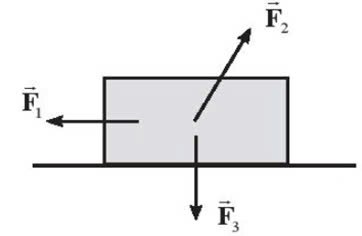
\includegraphics[scale=0.3]{../figs/LTTHPT-TOPIC3-1}}
	\loigiai{}
\end{ex}
% ===================================================================
\begin{ex}
	Một vận động viên cử tạ nâng quả tạ khối lượng \SI{200}{\kilogram} từ mặt đất lên độ cao \SI{1.5}{\meter}. Lấy gia tốc trọng trường là $g=\SI{9.8}{\meter/\second^2}$. Độ tăng thế năng của tạ là
	\choice
	{\SI{1962}{\joule}}
	{\True \SI{2940}{\joule}}
	{\SI{800}{\joule}}
	{\SI{3000}{\joule}}
	\loigiai{
	$\Delta W=W_{t2}-W_{t1}=mg\left(h_2-h_1\right)=\left(\SI{200}{\kilogram}\right)\cdot\left(\SI{9.8}{\meter/\second^2}\right)\cdot\left(\SI{1.5}{\meter}\right)=\SI{2940}{\joule}.$
	}
\end{ex}
% ===================================================================
\begin{ex}
	\immini{Quả bóng nhỏ được ném với vận tốc ban đầu \SI{4}{\meter / \second} theo phương ngang ra khỏi mặt bàn ở độ cao \SI{1}{\meter} so với mặt sàn. Lấy $g=\SI{9.81}{\meter / \second\squared}$ và bỏ qua mọi ma sát. Tính vận tốc của quả bóng khi nó chạm sàn. 
		\choice
		{\SI{4.52}{\meter/\second}}
		{\SI{9.16}{\meter/\second}}
		{\SI{7.25}{\meter/\second}}
		{\True \SI{5.97}{\meter/\second}}}{\vspace{-0.5cm}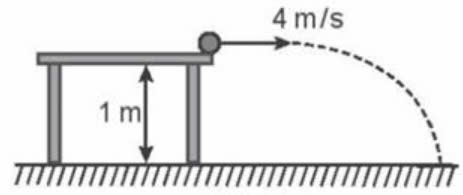
\includegraphics[scale=0.3]{../figs/LTTHPT-TOPIC3-4}}
	\loigiai{
	Chọn gốc thế năng tại mặt đất.\\
	Áp dụng định luật bảo toàn cơ năng:
	$$\dfrac{1}{2}mv^2_0+mgh=\dfrac{1}{2}mv^2_{\text{cđ}}\Rightarrow v_{\text{cđ}}=\sqrt{v^2_0+2gh}=\sqrt{\left(\SI{4}{\meter/\second}\right)^2+2\cdot\left(\SI{9.81}{\meter/\second^2}\right)\cdot\left(\SI{1}{\meter}\right)}\approx\SI{5.97}{\meter/\second}.$$
	}
\end{ex}
% ===================================================================
\begin{ex}
	Một học sinh ném một vật có khối lượng $\SI{200}{\gram}$ theo phương thẳng đứng lên cao với tốc độ ban đầu $\SI{8}{\meter / \second}$ từ độ cao $\SI{8}{\meter}$ so với mặt đất. Lấy $g=\SI{10}{\meter / \second\squared}$. Nếu có lực cản không khí với  độ lớn \SI{5}{\newton} tác dụng thì độ cao cực đại mà vật đạt được là bao nhiêu? 
	\choice
	{\True $\SI{8.56}{\meter}$}
	{$\SI{7.42}{\meter}$}
	{$\SI{4.81}{\meter}$}
	{$\SI{2.13}{\meter}$}
	\loigiai{
		Áp dụng biến thiên cơ năng:
		\begin{eqnarray*}
			&&W_0=W+\left|A_c\right|\\
			&\Rightarrow& \dfrac{1}{2}mv^2_0+mgh=mgh_{\max}+F_c\cdot\left(h_{\max}-h\right)\\
			&\Leftrightarrow& \dfrac{1}{2}\cdot\left(\SI{0.2}{\kilogram}\right)\cdot\left(\SI{8}{\meter/\second}\right)^2+\left(\SI{0.2}{\kilogram}\right)\cdot\left(\SI{10}{\meter/\second^2}\right)\cdot\left(\SI{8}{\meter}\right)=\left(\SI{0.2}{\kilogram}\right)\cdot\left(\SI{10}{\meter/\second^2}\right)\cdot h_{\max}+5\cdot\left(h_{\max}-\SI{8}{\meter}\right)\\
			&\Rightarrow& h_{\max}\approx\SI{8.91}{\meter}.
		\end{eqnarray*}
	\textbf{\color{red} Đáp án A là gần nhất, lỗi kĩ thuật \LARGE{\smiley}}
	}
\end{ex}
% ===================================================================
\begin{ex}
	\immini{Hình bên biểu diễn sự phụ thuộc thế năng và động năng của một chất điểm rơi tự do theo thời gian $t$. Động năng của chất điểm tại thời điểm chất điểm có thế năng bằng $\SI{8}{\joule}$ là
		\choice
		{$\SI{2}{\joule}$}
		{\True $\SI{4}{\joule}$}
		{$\SI{6}{\joule}$}
		{$\SI{3}{\joule}$}
	}	
	{\vspace{-0.5cm}\begin{tikzpicture}  
			\begin{axis}[  ultra thick,yscale=0.5,
				xmin=0,  
				xmax=7,  
				xtick=\empty,
				ytick={0,6,8},
				ymin=0,  
				ymax=14, 
				samples=300,
				xticklabels=\empty,
				xlabel=$\xsi{t}{\left(\si{\second}\right)}$, 		ylabel=$\xsi{W_{\text{đ}}, W_{\mathrm{t}}}{\left(\si{\joule}\right)}$,
				axis lines=center, 
				every axis y label/.style={at=(current axis.above origin),anchor=south},  
				every axis x label/.style={at=(current axis.right of origin),anchor=west},  ]
				\draw[line width=1pt, dashed] (axis cs: 0,8)--(axis cs: 3.266,8)--(axis cs: 3.266,0);
				\draw[line width=1pt, dashed] (axis cs: 0,6)--(axis cs: 4,6)--(axis cs: 4,0);
				\draw[line width=1pt, dashed] (axis cs: 0,12)--(axis cs: 5.6569,12)--(axis cs: 5.6569,0);
				\addplot [line width=1.5pt, red, smooth, domain=0:5.657] {12-3*x^2/8} node[above right] {$W_{\mathrm{t}}$};  
				\addplot [line width=1.5pt, blue, smooth, domain=0:5.657] {3*x^2/8} node[right] {$W_{\text{đ}}$}; 
				\coordinate (O) at (axis cs: 0,0);
			\end{axis}  
			\node[below left] at (O) {0};
	\end{tikzpicture}}
	\loigiai{
	Nhận thấy khi động năng bằng thế năng thì $W_{\mathrm{t}}=W_{\text{đ}}=\SI{6}{\joule}\Rightarrow W=2W_{\mathrm{t}}=\SI{12}{\joule}$.\\
	Tại $W'_{\mathrm{t}}=\SI{8}{\joule}\Rightarrow W'_{\text{đ}}=W-W'_{\mathrm{t}}=12-8=\SI{4}{\joule}$.
	}
\end{ex}
\Closesolutionfile{ans}
\section{Câu trắc nghiệm đúng/sai} 
\textit{Thí sinh trả lời từ câu 1 đến câu 4. Trong mỗi ý \textbf{a)}, \textbf{b)}, \textbf{c)}, \textbf{d)} ở mỗi câu, thí sinh chọn đúng hoặc sai}
\setcounter{ex}{0}\\
\Opensolutionfile{ans}[ans/D10-GK-HK2-003-TF]
% ===================================================================
\begin{ex}
	Vật nặng \SI{2}{\kilogram} trượt từ đỉnh dốc với tốc độ ban đầu $\SI{2}{\meter / \second}$ xuống chân dốc, dốc nghiêng một góc $\SI{30}{\degree}$ so với phương ngang. Vật đạt tốc độ $\SI{4}{\meter / \second}$ khi đến chân dốc, biết dốc dài $\SI{8}{\meter}$, lấy $g=\SI{9.81}{\meter / \second \squared}$.
	\choiceTF
	{\True Công của trọng lực trong quá trình trên là $\SI{78.48}{\joule}$}
	{\True Gia tốc của vật là $\SI{0.75}{\meter / \second \squared}$}
	{Công của lực ma sát trong quá trình trên là $\SI{-8.5}{\joule}$}
	{Hệ số ma sát trượt trên mặt phẳng nghiêng là $\SI{0.4}{}$}
	\loigiai{
		\begin{enumerate}[label=\alph*)] %alph=> arabic nếu muốn sử dụng số
			\item Đúng. $W_P=mgh\cos\SI{0}{\degree}=\SI{78.48}{\joule}$
			\item Đúng. $a=\dfrac{v^2-v_0^2}{2s}=\SI{0.75}{\meter / \second}$
			\item Sai. Áp dụng biến thiên cơ năng: $W_{\mathrm{A}}=W_{\mathrm{B}}+\left|A_{F_{\mathrm{ms}}}\right|\Leftrightarrow mgh_{\mathrm{A}}+\dfrac{1}{2}mv^2_{\mathrm{A}}=mgh_{\mathrm{B}}+\dfrac{1}{2}mv^2_{\mathrm{B}}+\left|A_{F_{\mathrm{ms}}}\right|$.\\
			Thay $m=\SI{2}{\kilogram}$, $h_{\mathrm{A}}=L\sin\theta=\SI{4}{\meter}$, $v_{\mathrm{A}}=\SI{2}{\meter/\second}$, $h_{\mathrm{B}}=0$; $v_{\mathrm{B}}=\SI{4}{\meter}$ thì thu được $\left|A_{F_{ms}}\right|=\SI{66.48}{\joule}\Rightarrow A_{F_{ms}}=\SI{-66.48}{\joule}$.
			\item Sai. $\mu=\dfrac{-A_{F_{ms}}}{mg\cos\theta}=\SI{0.061}{}$
		\end{enumerate}
	}
\end{ex}
% ===================================================================
\begin{ex}
	Xét tính đúng/sai của các phát biểu sau
	\choiceTF
	{\True Cơ năng bằng tổng động năng và thế năng của vật}
	{Năng lượng và công suất có cùng đơn vị đo}
	{Thế năng trọng trường của một vật phụ thuộc vào tốc độ chuyển động của vật}
	{\True Động năng của vật là dạng năng lượng vật có được do chuyển động}
	\loigiai{
		
	}
\end{ex}
% ===================================================================
\begin{ex}
	Hình bên mô tả các vị trí khác nhau của tàu lượn siêu tốc
	\immini{
		\choiceTF
		{Khi ở vị trí (1), thế năng trọng trường của tàu lượn đang chuyển hoá thành động năng của nó}
		{\True Vị trí (2) là vị trí tàu lượn có thế năng trọng trường lớn nhất}
		{Thế năng trọng trường của tàu lượn ở vị trí (5) lớn hơn vị trí (3)}
		{Ở vị trí (4) tàu lượn có động năng nhỏ nhất}}
	{\vspace{0.5cm}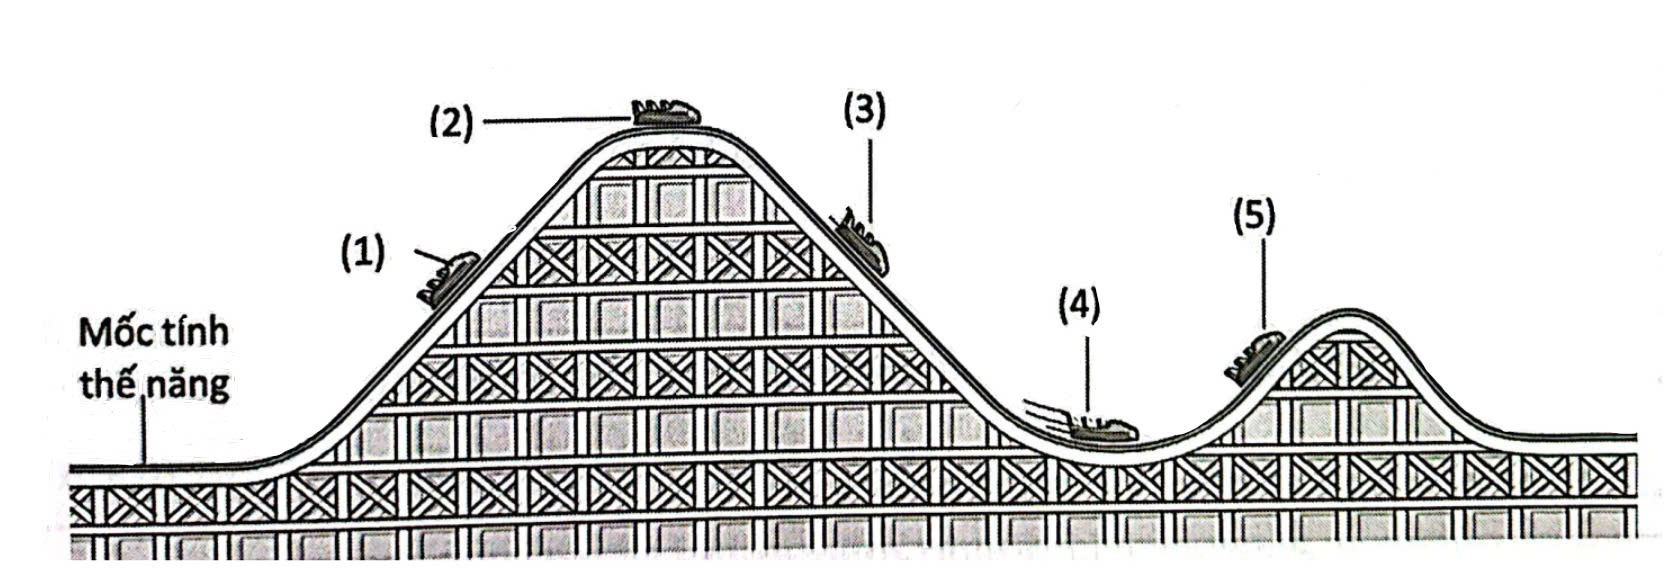
\includegraphics[scale=0.13]{../figs/LTTHPT-TOPIC3-17}}
	\loigiai{
		
	}
\end{ex}

% ===================================================================
\begin{ex}
	\immini{Một người đàn ông đẩy một thùng hàng có khối lượng $\SI{92}{\kilogram}$ với tốc độ $v=\SI{0.85}{\meter / \second}$ thì gặp một đoạn sàn thô ráp có chiều dài $\ell=\SI{0.65}{\meter}$ (hình bên). Hệ số ma sát trượt giữa thùng hàng với mặt sàn thô ráp là $\mu_t=\SI{0.358}{}$ và người này tác dụng một lực nằm ngang không đổi có độ lớn $\SI{275}{\newton}$ lên thùng hàng. Lấy $g=\SI{9.81}{\meter/\second\squared}$.
	}
	{\vspace{-0.5cm}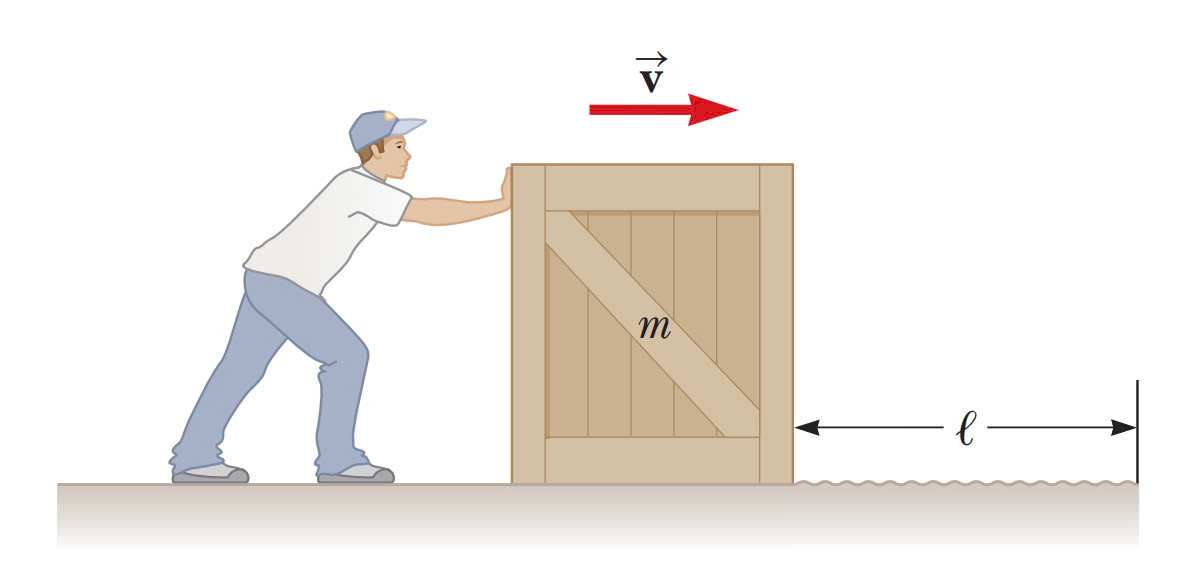
\includegraphics[scale=0.13]{../figs/LTTHPT-TOPIC3-18}}
	\choiceTF
	{Lực ma sát trong đoạn $\ell$ có độ lớn $\SI{200}{\newton}$}
	{Công của tổng hợp lực tác dụng lên thùng làm tăng động năng của thùng}
	{Trong quá trình chuyển động, cơ năng của thùng hàng được bảo toàn}
	{\True Tốc độ của thùng khi đến cuối đoạn sàn thô ráp là $\SI{0.21}{\meter/\second}$}
	\loigiai{
		\begin{enumerate}[label=\alph*)] %alph=> arabic nếu muốn sử dụng số
			\item Sai. $F_{ms}=\mu_tmg=\SI{323}{\newton}$.
			\item Sai. Lực ma sát lớn hơn lực đẩy trên phương ngang nên vật chuyển động chậm dần $\Rightarrow$ động năng giảm dần.
			\item Sai. Chịu tác dụng của lực đẩy và lực ma sát không phải là lực thế nên cơ năng không bảo toàn
			\item Đúng. Áp dụng định lý động năng:
			\begin{eqnarray*}
				&&W_{\text{đ2}} - W_{\text{đ1}}=A_{F_{ms}}+A_{F}\\
				&\Leftrightarrow&\dfrac{1}{2}mv^2_2-\dfrac{1}{2}mv^2_2=F_{ms}\cdot\ell\cos\SI{180}{\degree}+F\cdot\ell\cos\SI{0}{\degree}\\
				&\Leftrightarrow&\dfrac{1}{2}\cdot\left(\SI{92}{\kilogram}\right)\cdot v^2_2-\dfrac{1}{2}\cdot\left(\SI{92}{\kilogram}\right)\cdot \left(\SI{0.85}{\meter/\second}\right)^2=\left(\SI{323}{\newton}\right)\cdot\left(\SI{0.65}{\meter}\right)\cdot\cos\SI{180}{\degree}+\left(\SI{275}{\newton}\right)\cdot\left(\SI{0.65}{\meter}\right)\cdot\cos\SI{0}{\degree}\\
				&\Rightarrow& v_2=\SI{0.21}{\meter / \second}.
			\end{eqnarray*}
		\end{enumerate}
	}
\end{ex}
\Closesolutionfile{ans}
\section{Tự luận} 
\setcounter{ex}{0}
\Opensolutionfile{ans}[ans/D10-GK-HK2-003-TL]
% ===============================================================
\begin{ex}
	Súng ngắn Makarov có độ dài nòng súng \SI{93.5}{\milli\meter}. Súng dùng loại đạn có tốc độ đầu nòng $\SI{315}{\meter / \second}$ có khối lượng mỗi viên đạn là $\SI{7.45}{\gram}$. Lực đẩy trung bình của thuốc súng tác dụng lên viên đạn là bao nhiêu newton $\left(\si{\newton}\right)$? \textit{(Kết quả làm tròn đến chữ số hàng đơn vị).}
	\loigiai{
		Áp dụng định lý động năng:
		\begin{eqnarray*}
			&&W_{\text{đ2}} - W_{\text{đ1}}=A_{F}\\
			&\Leftrightarrow&\dfrac{1}{2}mv^2_2-\dfrac{1}{2}mv^2_2=F\cdot\ell\cos\SI{0}{\degree}\\
			&\Leftrightarrow&\dfrac{1}{2}\cdot\left(\SI{7.45e-3}{\kilogram}\right)\cdot \left(\SI{315}{\meter/\second}\right)^2-0=F\cdot\left(\SI{93.5E-3}{\meter}\right)\cdot\cos\SI{0}{\degree}\\
			&\Rightarrow& F\approx\SI{3953}{\newton}.
		\end{eqnarray*}
	}
\end{ex}
% ===============================================================
\begin{ex}
	Một vật khối lượng $m=\SI{200}{\gram}$ được ném thẳng đứng lên trên với tốc độ ban đầu $v_0=\SI{15.0}{\meter/\second}$ từ một điểm có độ cao $h=\SI{20.0}{\meter}$ so với mặt đất nằm ngang. Biết gia tốc rơi tự do tại nơi ném vật là $g=\SI{9.8}{\meter/\second^2}$. Vật đạt độ cao cực đại so với mặt đất là $H=\SI{30.0}{\meter}$ và tiếp đất với tốc độ $v=\SI{22.0}{\meter/\second}$.
	\begin{enumerate}[label=\alph*)]
		\item Tính cơ năng ban đầu của vật.
		\item Tính cơ năng của vật khi nó đạt độ cao cực đại so với mặt đất và khi nó tiếp đất.
		\item Tính công của lực cản không khí tác dụng lên vật trong giai đoạn vật bay lên và giai đoạn vật rơi xuống.
	\end{enumerate}
	\loigiai{Chọn gốc thế năng tại mặt đất.
		\begin{enumerate}[label=\alph*)]
			\item Cơ năng ban đầu của vật: $W_0=mgh+\dfrac{1}{2}mv^2_0=\SI{61.7}{\joule}$.
			\item Cơ năng của vật khi đạt độ cao cực đại: $W_1=mgH=\SI{58.8}{\joule}$.\\
			Cơ năng của vật khi nó tiếp đất: $W_2=\dfrac{1}{2}mv^2_{\text{cđ}}=\SI{48.4}{\joule}$.
			\item Công của lực cản không khí tác dụng lên vật khi bay lên:
			$$W_0=W_1+\left|A_{F_c}\right|\Rightarrow\left|A_{F_c}\right|=\SI{2.9}{\joule}\Rightarrow A_{F_c}=\SI{-2.9}{\joule}.$$
			Công của lực cản không khí tác dụng lên vật khi rơi xuống:
			$$W_1=W_2+\left|A'_{F_c}\right|\Rightarrow\left|A'_{F_c}\right|=\SI{10.4}{\joule}\Rightarrow A_{F_c}=\SI{-10.4}{\joule}.$$
		\end{enumerate}
	}
\end{ex}
% =======================================================================================================================================================
\begin{ex}
	\immini{Vật nặng \SI{5}{\kilogram} được coi là chất điểm được đẩy lên một mặt phẳng nghiêng với vận tốc ban đầu $v_i=\SI{8}{\meter / \second}$. Vật dừng lại sau khi di chuyển được một đoạn $d=\SI{5}{\meter}$ dọc theo mặt phẳng nghiêng, với góc nghiêng $\theta=\SI{30}{\degree}$ so với phương ngang.  Lấy $g=\SI{9.81}{\meter / \second\squared}$.\begin{enumerate}[label=\alph*)]
			\item Xác định độ lớn của lực ma sát tác dụng lên vật.
			\item Tốc độ của vật sau khi đi được đoạn $d=\SI{3}{\meter}$ là bao nhiêu?
	\end{enumerate}}
	{\vspace{-0.5cm}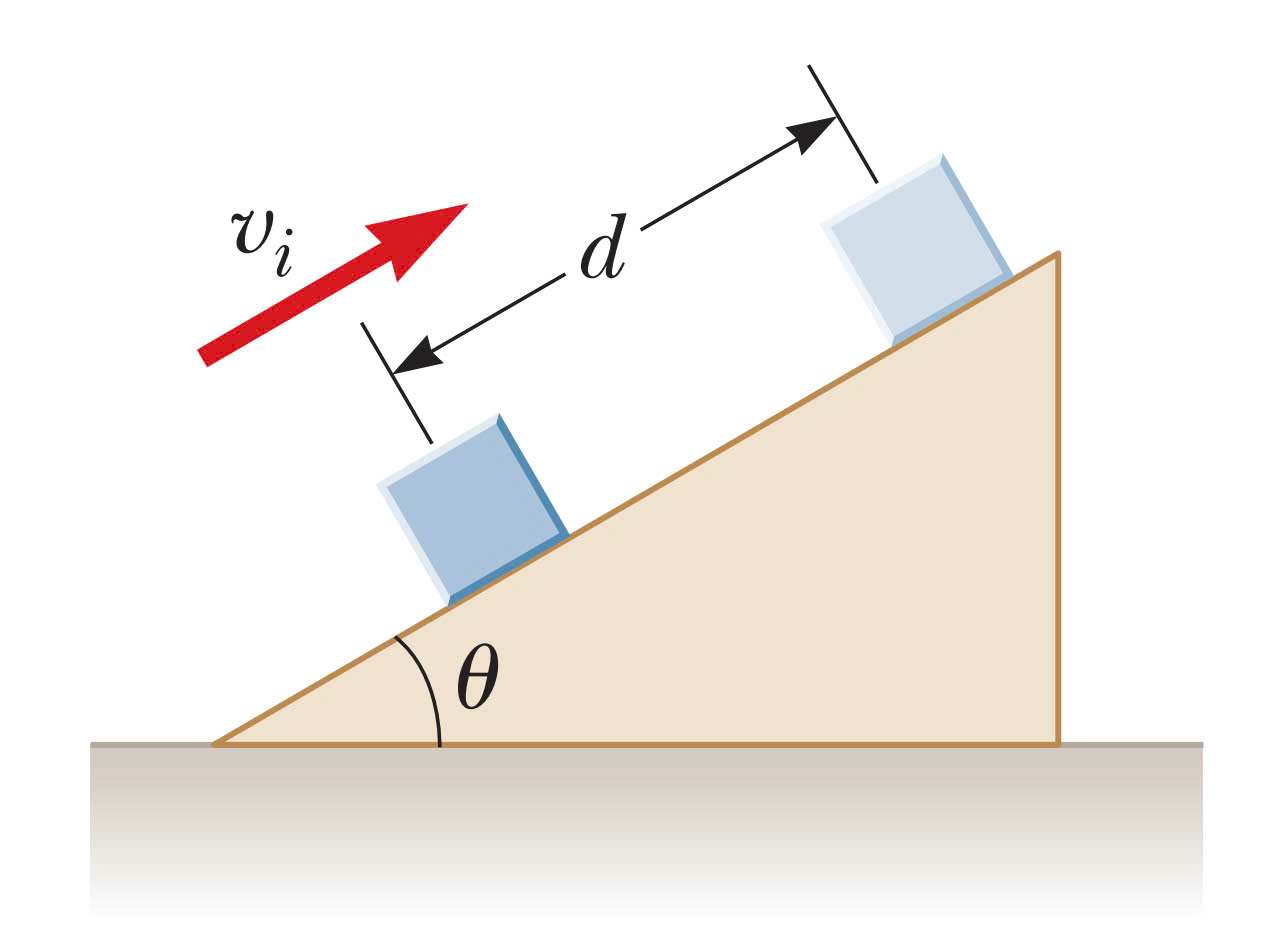
\includegraphics[scale=0.1]{../figs/LTTHPT-TOPIC3-2}}
	
	\loigiai{
	\begin{enumerate}[label=\alph*)]
		\item Áp dụng biến thiên cơ năng:
		\begin{eqnarray*}
			&&\dfrac{1}{2}mv^2_i+0=mgh+\left|A_{F_{ms}}\right|\\
			&\Leftrightarrow& \dfrac{1}{2}\cdot\left(\SI{5}{\kilogram}\right)\cdot\left(\SI{8}{\meter/\second}\right)^2=\left(\SI{5}{\kilogram}\right)\cdot\left(\SI{9.81}{\meter/\second^2}\right)\cdot\left(\SI{5}{\meter}\right)\cdot\sin{\SI{30}{\degree}}+F_{ms}\cdot\left(\SI{5}{\meter}\right)\\
			&\Rightarrow&F_{ms}=\SI{7.475}{\newton}.
		\end{eqnarray*}
		\item Áp dụng biến thiên cơ năng:
		\begin{eqnarray*}
			&&\dfrac{1}{2}mv^2_i+0=mgh'+\dfrac{1}{2}mv^2+\left|A_{F_{ms}}\right|\\
			&\Leftrightarrow& \dfrac{1}{2}\cdot\left(\SI{5}{\kilogram}\right)\cdot\left(\SI{8}{\meter/\second}\right)^2=\left(\SI{5}{\kilogram}\right)\cdot\left(\SI{9.81}{\meter/\second^2}\right)\cdot\left(\SI{3}{\meter}\right)\cdot\sin{\SI{30}{\degree}}+\dfrac{1}{2}\cdot\left(\SI{5}{\kilogram}\right)\cdot v^2+\left(\SI{7.475}{\meter}\right)\cdot\left(\SI{3}{\meter}\right)\\
			&\Rightarrow&v\approx\SI{5.06}{\meter/\second}.
		\end{eqnarray*}
	\end{enumerate}
	}
\end{ex}

\Closesolutionfile{ans}
\begin{center}
	\textbf{--- HẾT ---}
\end{center}